\documentclass[11pt]{article}
\usepackage{microtype}
\usepackage{graphicx}
\usepackage{wrapfig}
\usepackage{url}
\usepackage{wrapfig}
\usepackage{color}
\usepackage{marvosym}
\usepackage{enumerate}
\usepackage{subfigure}
\usepackage{tikz}
\usepackage[fleqn]{amsmath}
\DeclareMathOperator*{\argmax}{arg\,max}
\DeclareMathOperator*{\argmin}{arg\,min}
\usepackage{amssymb}
\usepackage{hyperref}
\usepackage[many]{tcolorbox}
\usepackage{lipsum}
\usepackage{float}
\usepackage{trimclip}
\usepackage{listings}
\usepackage{environ}% http://ctan.org/pkg/environ
\usepackage{wasysym}
\usepackage{array}


\oddsidemargin 0mm
\evensidemargin 5mm
\topmargin -20mm
\textheight 240mm
\textwidth 160mm

\newcommand{\vwi}{{\bf w}_i}
\newcommand{\vw}{{\bf w}}
\newcommand{\vx}{{\bf x}}
\newcommand{\vy}{{\bf y}}
\newcommand{\vxi}{{\bf x}_i}
\newcommand{\yi}{y_i}
\newcommand{\vxj}{{\bf x}_j}
\newcommand{\vxn}{{\bf x}_n}
\newcommand{\yj}{y_j}
\newcommand{\ai}{\alpha_i}
\newcommand{\aj}{\alpha_j}
\newcommand{\X}{{\bf X}}
\newcommand{\Y}{{\bf Y}}
\newcommand{\vz}{{\bf z}}
\newcommand{\msigma}{{\bf \Sigma}}
\newcommand{\vmu}{{\bf \mu}}
\newcommand{\vmuk}{{\bf \mu}_k}
\newcommand{\msigmak}{{\bf \Sigma}_k}
\newcommand{\vmuj}{{\bf \mu}_j}
\newcommand{\msigmaj}{{\bf \Sigma}_j}
\newcommand{\pij}{\pi_j}
\newcommand{\pik}{\pi_k}
\newcommand{\D}{\mathcal{D}}
\newcommand{\el}{\mathcal{L}}
\newcommand{\N}{\mathcal{N}}
\newcommand{\vxij}{{\bf x}_{ij}}
\newcommand{\vt}{{\bf t}}
\newcommand{\yh}{\hat{y}}
\newcommand{\code}[1]{{\footnotesize \tt #1}}
\newcommand{\alphai}{\alpha_i}
\newcommand{\defeq}{\overset{\text{def}}{=}}
\renewcommand{\vec}[1]{\mathbf{#1}}


\bgroup
\def\arraystretch{1.5}
\newcolumntype{x}[1]{>{\centering\arraybackslash\hspace{0pt}}p{#1}}
\newcolumntype{z}[1]{>{\centering\arraybackslash}m{#1}}

%Arguments are 1 - height, 2 - box title
\newtcolorbox{textanswerbox}[2]{%
 width=\textwidth,colback=white,colframe=blue!30!black,floatplacement=H,height=#1,title=#2,clip lower=true,before upper={\parindent0em}}

 \newtcolorbox{eqanswerbox}[1]{%
 width=#1,colback=white,colframe=black,floatplacement=H,height=3em,sharp corners=all,clip lower=true,before upper={\parindent0em}}

 %Arguments are 1 - height, 2 - box title
 \NewEnviron{answertext}[2]{
        \noindent
        \marginbox*{0pt 10pt}{
        \clipbox{0pt 0pt 0pt 0pt}{
        \begin{textanswerbox}{#1}{#2}
        \BODY
        \end{textanswerbox}
        }
        }
}

%Arguments are 1 - height, 2 - box title, 3 - column definition
 \NewEnviron{answertable}[3]{
        \noindent
        \marginbox*{0pt 10pt}{
        \clipbox{0pt 0pt 0pt 0pt}{
        \begin{textanswerbox}{#1}{#2}
                \vspace{-0.5cm}
                        \begin{table}[H]
                        \centering
                        \begin{tabular}{#3}
                                \BODY
                        \end{tabular}
                        \end{table}
        \end{textanswerbox}
        }
        }
}

 %Arguments are 1 - height, 2 - box title, 3 - title, 4- equation label, 5 - equation box width
 \NewEnviron{answerequation}[5]{
        \noindent
        \marginbox*{0pt 10pt}{
        \clipbox{0pt 0pt 0pt 0pt}{
        \begin{textanswerbox}{#1}{#2}
                \vspace{-0.5cm}
                        \begin{table}[H]
                        \centering
                \renewcommand{\arraystretch}{0.5}% Tighter

                        \begin{tabular}{#3}
                                #4 =	&
                        \clipbox{0pt 0pt 0pt 0pt}{

                        \begin{eqanswerbox}{#5}
                                $\BODY$
                        \end{eqanswerbox}
                        } \\
                        \end{tabular}
                        \end{table}

        \end{textanswerbox}
        }
        }
}

 %Arguments are 1 - height, 2 - box title
 \NewEnviron{answerderivation}[2]{
        \noindent
        \marginbox*{0pt 10pt}{
        \clipbox{0pt 0pt 0pt 0pt}{
        \begin{textanswerbox}{#1}{#2}
        \BODY
        \end{textanswerbox}
        }
        }
}

\newcommand{\Checked}{{\LARGE \XBox}}%
\newcommand{\Unchecked}{{\LARGE \Square}}%
\newcommand{\TextRequired}{{\textbf{Place Answer Here}}}%
\newcommand{\EquationRequired}{\textbf{Type Equation Here}}%


\newcommand{\answertextheight}{5cm}
\newcommand{\answertableheight}{4cm}
\newcommand{\answerequationheight}{2.5cm}
\newcommand{\answerderivationheight}{14cm}

\newcounter{QuestionCounter}
\newcounter{SubQuestionCounter}[QuestionCounter]
\setcounter{SubQuestionCounter}{1}

\newcommand{\subquestiontitle}{Question \theQuestionCounter.\theSubQuestionCounter~}
\newcommand{\newquestion}{\stepcounter{QuestionCounter}\setcounter{SubQuestionCounter}{1}\newpage}
\newcommand{\newsubquestion}{\stepcounter{SubQuestionCounter}}

\DeclareMathOperator{\rank}{rank}
\DeclareMathOperator{\indices}{indices}
\DeclareMathOperator{\Bernoulli}{Bernoulli}
\DeclareMathOperator{\Bin}{Bin}
\DeclareMathOperator{\E}{E}
\DeclareMathOperator{\Var}{Var}
\DeclareMathOperator{\Cov}{Cov}

\lstset{language=[LaTeX]TeX,basicstyle=\ttfamily\bf}

\pagestyle{myheadings}
\markboth{Homework 3}{Fall 2021 CS 475/675 Machine Learning: Homework 3}

\title{CS 475 Machine Learning: Homework 3 Analytical \\
(35 points)\\
\Large{Assigned: Friday, September 24, 2021} \\
\Large{Due: Friday, October 8, 2021, 11:59 pm US/Eastern}}
\author{Partner 1: NAME (JHED), Partner 2:  NAME (JHED)}
\date{}

\begin{document}
\maketitle
\thispagestyle{headings}

\section*{Instructions }
We have provided this \LaTeX{} document for turning in this homework. We give you one or more boxes to answer each question.  The question to answer for each box will be noted in the title of the box.  You can change the size of the box if you need more space.\\

{\bf Other than your name, do not type anything outside the boxes. Leave the rest of the document unchanged.}\\


\textbf{
%Do not change any formatting in this document, or we may be unable to
  %grade your work. This includes, but is not limited to, the height of
  %textboxes, font sizes, and the spacing of text and tables.  Additionally,
  Do
  not add text outside of the answer boxes.  You are allowed to make boxes larger if needed.
  % Entering your answers are the only
  %changes allowed.
  }\\


\textbf{We strongly recommend you review your answers in the generated PDF to
  ensure they appear correct. We will grade what appears in the answer boxes in
  the submitted PDF, NOT the original latex file.}

% \section*{ Notation}
% {
% \centering
% \smallskip\begin{tabular}{r l}
% \(\vec{x_i}\) & One input data vector. \(\vec{x_i}\) is \(M\) dimensional.
% \(\vec{x_i} \in \mathbb{R}^{1 \times M}\).  \\ &
% We assume $\vec{x_i}$ is augmented with a  $1$ to include a bias term. \\ \\
% \(\vec{X}\) & 	A matrix of concatenated \(\vec{x_i}\)'s. There are \(N\) input vectors, so \(\vec{X} \in \mathbb{R}^{N \times M}\) \\ \\
% \(y_i\) & The true label for input vector \(\vec{x_i}\). In regression problems, \(y_i\) is continuous. \\ & In general ,\(y_i\) can be a vector, but for now we assume it's a scalar: \(y_i \in \mathbb{R}^1\). \\ \\

% \(\vec{y}\) & 	A vector of concatenated \(y_i\)'s. There are \(N\) input vectors, so \(\vec{y} \in \mathbb{R}^{N \times 1}\) \\ \\

% \(\vec{w}\) & A weight vector. We are trying to learn the elements of \(\vec{w}\). \\
% & \(\vec{w}\) is the same number of elements as \(\vec{x_i}\) because we will end up computing \\
% & the dot product \(\vec{x_i} \cdot \vec{w}\). \\
% & \(\vec{w} \in \mathbb{R}^{M \times 1}\). We assume the bias term is included in \(\vec{w}\). \\ \\

% \(h(\vec(x))\) & The true regression function that describes the data. \\ \\
 
% i.i.d. & Independently and identically distributed. \\ \\

% Bias-variance  & We can write \(E_D[(f(x, D) - h(x))^2]\) = \\
% decomposition  & \((E_D[f(x, D) - h(x))^2 + E_D[(f(x, D) - E_D[f(x, D)])^2]\) \\
%                             & where the first term is the bias squared, and the second term is the variance.\\ \\

%  Notes: & In general, a lowercase letter (not boldface), $a$, indicates a scalar. \\
%   & A boldface lowercase letter, $\vec{a}$, indicates a vector. \\  &  A boldface uppercase letter, $\vec{A}$, indicates a matrix. \\
% \end{tabular}
% }
%%%%%%%%%%%%%%%%%%%%%%%%%%%%%%%%%%%%%%%%%%%%%%%%%%%%%%%%%%%%%%%%%%%%%%%%%%%%%%%%


% -----------------------------------------------------------

\pagebreak
\section{Neural Networks}

\newcommand{\norm}[1]{\left\lVert#1\right\rVert}

\begin{enumerate}

\item Consider a neural network model with $n$ layers, where the vertex for each internal layer is determined by a ReLU activation function applied to a weighted combination of vertices of the previous layer, while the output layer is the given by a weighted linear function of the outputs of the previous layer (without ReLU).

\begin{itemize}

\item[(a)] Show that if we replace all ReLU units by the identity function $f(x) = x$, the resulting neural network yields a linear regression model of the inputs.

\item[(b)] Is there a unique loss minimizer setting of weights for this model?  Explain.

\end{itemize}

% Problem 1.1
\begin{answertext}{20cm}{}

(a) \\
In a neural network, the j-th output at the i-th layer is given by $ x_{ij} = g(\beta_{0} + \vec{\beta^{T}_{i - 1}}\vec{x_{i-1}}) $. \\
In this case, the activation function is $ g(x) = x $. \\
Thus, $ x_{ij} = \beta_{0} + \vec{\beta^{T}_{i - 1}}\vec{x_{i-1}} $. The output from the previous layer will be exactly the input for the next layer. \\
We want to show that if the input of a layer is a linear combination of model inputs, then the output of this layer is also a linear combination of model inputs. \\
Let $ \vec{x_{i-1}} = \vec{\beta_{0,i-1}} + \vec{B_{i-1}}\vec{x_{0}} $, where $ \vec{x_{i-1}} $ is the vector of output from layer i-1,
$ \vec{\beta_{0,i-1}} $ is the vector of biases, $ \vec{B_{i-1}} $ is the matrix whose rows are the linear combination coefficients for each output of the layer,
and $ \vec{x_{0}} $ is the model inputs. \\
Then, for each output $ x_{ij} $ in layer i,
\begin{align*}
x_{ij} &= \beta_{0,ij} + \vec{\beta^{T}_{ij}}\vec{x_{i-1}} \\
&= \beta_{0,ij} + \vec{\beta^{T}_{ij}}(\vec{\beta_{0,i-1}} + \vec{B_{i-1}}\vec{x_{0}}) \\
&= (\beta_{0,ij} + \vec{\beta^{T}_{ij}}\vec{\beta_{0,i-1}}) + (\vec{\beta^{T}_{ij}}\vec{B_{i-1}})\vec{x_{0}}
\end{align*}
Which is a linear combination of $ \vec{x_{0}} $. \\
The whold neural model is but stacking of such layers. Since the each of model inputs is obviously a linear combination of itself, the model output is also a linear combination of the inputs. \\
\\
(b) \\
Assume that we are talking about the model discussed in part (a). \\
For an arbitrary type of loss, assume that we now have a setting of weights that minimizes the loss. If we now multiply all the $ \beta_{0} $ and $ \vec{\beta^{T}_{i-1}} $ in layer i-1 by $\lambda$, and divide all the $ \vec{\beta^{T}_{i}} $ in layer i by $\lambda$, the final output of the model will not change because all the layers are linear combinations of the previous layers. Thus, the modified weights also minimize the loss. Thus, loss minimizer setting of weights is not unique. We can prove this quickly: \\
\\
If $ \vec{x_{i-1}} = \lambda(\vec{\beta_{0,i-1}} + \vec{B_{i-1}}\vec{x_{0}}) $, $ x_{ij} = \beta_{0} + \frac{1}{\lambda}\vec{\beta^{T}_{i - 1}}\vec{x_{i-1}} $
\begin{align*}
x_{ij} &= \beta_{0,ij} + \frac{1}{\lambda}\vec{\beta^{T}_{ij}}\vec{x_{i-1}} \\
&= \beta_{0,ij} + \frac{1}{\lambda}\vec{\beta^{T}_{ij}}\lambda(\vec{\beta_{0,i-1}} + \vec{B_{i-1}}\vec{x_{0}}) \\
&= (\beta_{0,ij} + \vec{\beta^{T}_{ij}}\vec{\beta_{0,i-1}}) + (\vec{\beta^{T}_{ij}}\vec{B_{i-1}})\vec{x_{0}}
\end{align*}
Which does not change.

\end{answertext} 

\pagebreak

\item Consider a neural network with a single intermediate layer and a single output, where the the activation function for every vertex in the intermediate layer is the sigmoid function $\sigma(v) = \frac{1}{1 + \exp\{ - v \}}$ of a weighted linear combination of inputs, while the output is a weighted linear combination of the all the intermediate vertices, and all weights are non-negative.  Show that this model has a likelihood convex with respect to all weight parameters.

Hints:
\begin{itemize}
\item First show that the negative log likelihood for each intermediate layer vertex $v$ (viewed as the outcome), with the weighted combination of inputs for that vertex (viewed as a single feature $x$) is a convex function.  That is, show that:
{
\begin{align*}
h(x) = - v \log \sigma(x) - (1 - v) \log ( 1 - \sigma(x) )
\end{align*}
}
is convex in $x$.  You can do this by showing that the second derivative of this function with respect to $x$ is always non-negative.
\item Then, show that a composition of a linear function $g(w_1, \ldots, w_k)$ of several arguments and a convex function $h(x)$ that is convex in its single argument $x$ is convex in each argument.  That is, show that $h(g(w_1, \ldots, w_k))$ is convex in each $w_1, \ldots, w_k$.
\item Finally, show that a weighted combination of convex functions is also convex, if all weights are non-negative.
\end{itemize}

\begin{answertext}{10cm}{}


  
\end{answertext} 

\pagebreak

\item Assume there exist a setting of parameters for this model that minimizes the squared loss, such that at least two intermediate nodes have different weights feeding into their activation function.
Show that there exists more than one setting of parameters that minimizes the squared loss.  (This shows the parameters of this model are not identified).

\begin{answertext}{10cm}{}


  
\end{answertext} 

\pagebreak

\item
This question contains multiple parts. Please answer all of these parts in large the answer box following the question. (Feel free to increase the box for additional space.)

Consider the 2-layer neural network shown below. There are three input features $x_1$, $x_2$, and $x_3$ which get fed into one activation ($a_1$) from which a hidden value is computed ($h_1$). The non-linearities connecting activations to hidden values are \textbf{rectified linear units} $ReLU$: $h_1$ = $ReLU(a_1)$, with $ReLU(x) = 0$ if $x < 0$, and $ReLU(x) = x$ otherwise. The output unit takes 2 inputs: the hidden value $h_1$ and $x_1$.

\begin{figure}[htbp]
 \centerline{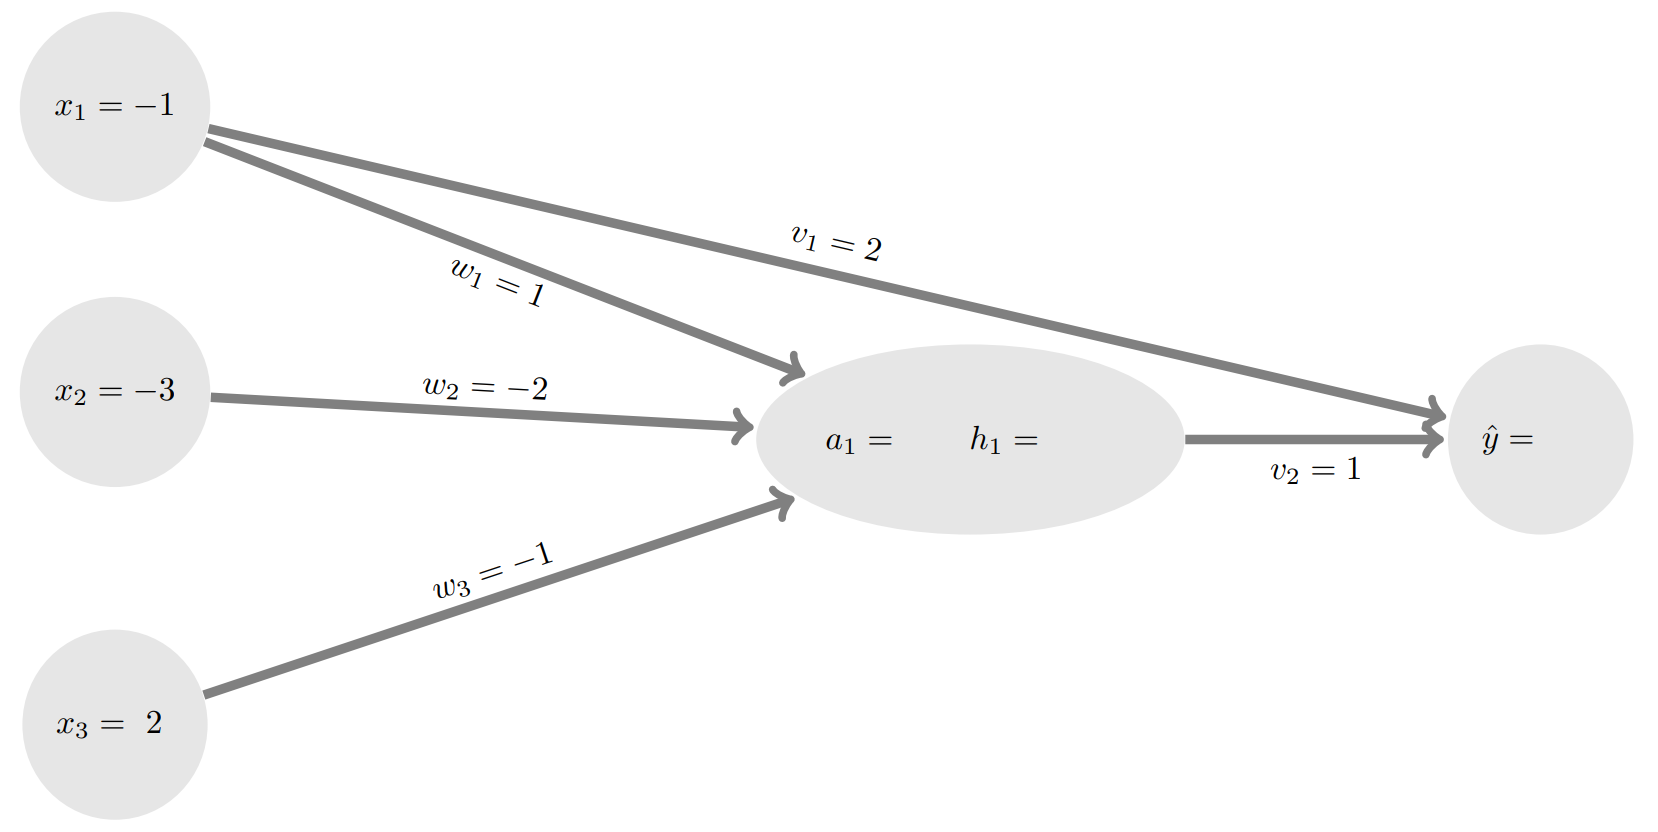
\includegraphics[scale=0.35]{grad_example.png}}
 \label{fig:backprop}
\end{figure}

\begin{enumerate}[(i) ]
    \item Execute forward propagation on this network, writing the appropriate values for $a_1$, $a_2$, $h_1$, $h_2$ and $\hat{y}$ in the figure above.
    \item Give the expression of $\hat{y}$ as a function of $x_1$, $x_2$, $x_3$, $w_1$, $w_2$, $w_3$, $v_1$, $v_2$ and the $ReLU(\cdot)$ function.
    \item The correct class for example $x = [x_1, x_2, x_3] = [-1, -3, -2]$ is $y = -1$. Please run the backpropagation algorithm to minimize the squared error loss $l = \frac{1}{2}(y - \hat{y})^2$ on this single example. Derive the mathematical expression of the gradients of the loss $l$ with respect to weights $w_1$, $w_2$, and $w_3$, and calculate its numerical value.
    \item Indicate how the value of each parameter below changes after the update: does it increase, decrease, or stay the same?
    \item Derive the update rule for parameters $v_1$ and $v_2$ when running the backpropagation algorithm on the same example $x$, with the squared loss $l$ and a step size $\eta = {1}{2}$. \textit{Hint: you will need to (1) derive the appropriate gradient, (2) evaluate the gradient, (3) update your guess for the parameter $\beta_{\text{new}}$ by subtracting the gradient times the step size from the old guess $\beta_{\text{old}}$.}
\end{enumerate}

\begin{answertext}{22cm}{}


  
\end{answertext} 

\end{enumerate}

% -----------------------------------------------------------
\pagebreak
\section{SVMs}

\begin{enumerate}

\item Consider 2D classification problem with 3 classes with the following training sample:\\\\\
\textbf{Class 1:} (0,1), (0,2), (1,1)\\
\textbf{Class 2:} (-2,0), (-1,0), (-1,-1)\\
\textbf{Class 3:} (2,0), (3,0), (2,-1)\\
\begin{enumerate}[(a)]
    \item 
    Explain how you would formulate an SVM model to solve this problem. (Hint: How many classifiers do you need?)\\
\begin{answertext}{5cm}{}  
\end{answertext} 
    \item
    Find $w$, $b$, and corresponding support vectors for each classifier. Please draw the plot.  You can take a screenshot or photo and use the \texttt{{\textbackslash}includegraphics\{\}} directive.\\
%\includegraphics{}
    \item
    Given a test sample, explain how to make a decision.\\
\begin{answertext}{5cm}{}
\end{answertext} 
\end{enumerate}

\end{enumerate}

\end{document}
